% Created 2018-06-20 Wed 23:48
\documentclass[presentation]{beamer}
\usepackage[latin1]{inputenc}
\usepackage[T1]{fontenc}
\usepackage{fixltx2e}
\usepackage{graphicx}
\usepackage{longtable}
\usepackage{float}
\usepackage{wrapfig}
\usepackage{rotating}
\usepackage[normalem]{ulem}
\usepackage{amsmath}
\usepackage{textcomp}
\usepackage{marvosym}
\usepackage{wasysym}
\usepackage{amssymb}
\usepackage{hyperref}
\tolerance=1000
\usetheme{default}
\author{bollu}
\date{\today}
\title{slides}
\hypersetup{
  pdfkeywords={},
  pdfsubject={},
  pdfcreator={Emacs 24.5.1 (Org mode 8.2.10)}}
\begin{document}

\maketitle
\begin{frame}{Outline}
\tableofcontents
\end{frame}

\begin{frame}[label=sec-1]{Proof outline}
\begin{itemize}
\item Algbra of polyhedra, $P(\mathbb{Q}^d)$
\item $[\text{ }] : \mathbb{Q}^d \rightarrow P(\mathbb{Q}^d)$
\item Existence of $\mathcal{F}: P(\mathbb{Q}^d) \rightarrow \mathbb{C}(x)$, such that:
\begin{itemize}
\item \mathcal{F} is linear
\item P is a polyhedra, then $\mathcal{F}([P]) = \sum_{\vec{m} \in P \cap \mathbb{Z}^d} (x^{\vec{m}} )$
\item $\mathcal{F}([\text{line}]) = 0$
\end{itemize}
\item $\mathcal{F}(P)(1) = \text{number of points in} P$
\item reduction: \mathcal{F} for cones gives full \mathcal{F}
\item reduction: \mathcal{F} for simple cones gives \mathcal{F} for cones
\end{itemize}
\end{frame}


\begin{frame}[label=sec-2]{Caveats}
\begin{itemize}
\item Do not understand subtleties of convergence arguments (how is evaluating at $\vec{1}$ correct?).
\item No intuition for LLL, Lattice reduction.
\end{itemize}
\end{frame}

\begin{frame}[label=sec-3]{Assuming $\mathcal{F}$ for cones, derive full $\mathcal{F}$: Part 1 (Polytopes)}
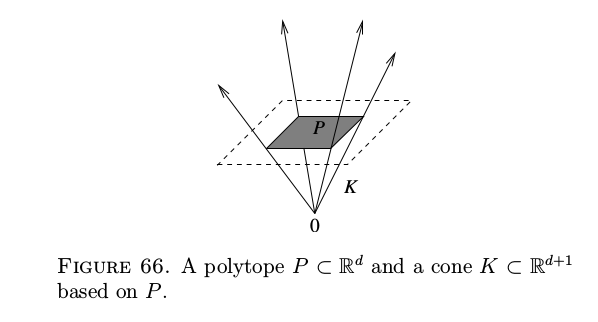
\includegraphics[width=.9\linewidth]{./res/polytope-as-cross-section-of-cone.png}
\begin{itemize}
\item Write polytope as intersection of hyperplane + cone.
\item $\mathcal{F}(\text{polytope}) = (\frac{d}{dx} \mathcal{F}(\text{cone}))(1)$
\end{itemize}
\end{frame}

\begin{frame}[label=sec-4]{Assuming $\mathcal{F}$ for cones, derive full $\mathcal{F}$: Part 2 (Lines)}
\begin{itemize}
\item Line = cone + cone - point.
\item Since line can be translated, $\forall \vec{x} \in L, L = \vec{x} + L$
\begin{itemize}
\item $\forall x \in L, \mathcal{F}(L) = \mathcal{F}(L) + \mathcal{F}(\vec{x})$
\item $\mathcal{F}(L) = 0$
\end{itemize}
\end{itemize}
\end{frame}


\begin{frame}[label=sec-5]{Assuming $\mathcal{F}$ for simple cone, derive for cone}
\begin{itemize}
\item inclusion exclusion: decompose cone into simple cones.
\end{itemize}
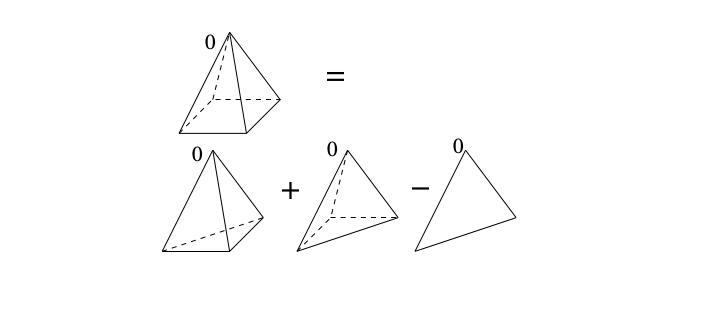
\includegraphics[width=.9\linewidth]{./res/cut-cone-into-simple-cones.png}
\end{frame}





\begin{frame}[label=sec-6]{References}
\begin{itemize}
\item Lattice Points, Polyhedra, and Complexity: Alexander Barvinok
\item Integer points in polyhedra: Alexander Barvinok
\end{itemize}
\end{frame}
% Emacs 24.5.1 (Org mode 8.2.10)
\end{document}
